\documentclass[8pt]{beamer}

\setbeamertemplate{background canvas}[vertical shading][bottom=cyan!10,top=blue!10]

\usetheme{Warsaw}
\usefonttheme[onlysmall]{structurebold}

% pour le fichiers .pdf
\usepackage{graphicx}
\usepackage{color}
% pour les fichiers .png
% \usepackage{pgf,pgfarrows}
% \usepackage{pgf,pgfarrows}
\usepackage{amsmath,amssymb}
\usepackage[latin1]{inputenc}
\usepackage[T1]{fontenc}
\usepackage[french]{babel}
\usepackage{textcomp}
\usepackage{Math_Notations}
\usepackage{multitoc}
\usepackage{mdwtab}
\setbeamercovered{dynamic}
\DeclareMathOperator*{\argmin}{argmin}

\title[OpenTURNS Developer training]{OpeTURNS Developer training: module development}
\author[R. Lebrun, copyright EADS 2011.]
{
  Trainer : R�gis LEBRUN\\
  EADS/IW/SE/AM\\
  regis.lebrun@eads.net
}



\date[March 22-25th 2011]
{
  Developers training \\

  \begin{center}
    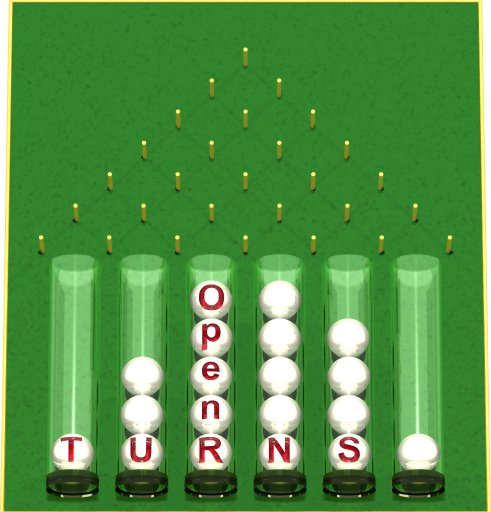
\includegraphics[height=2cm]{logoOT.jpg}
  \end{center}
}

\subject{OpenTURNS Developers Training}

% \part<presentation>{Corps de presentation}


\begin{document}

\frame{\titlepage}

% necessaire pour la table des matieres
\part{Main part}

%%%%%%%%%%%%%%%%%%%%%%%%%%%%%%%%%
% Navigation in the source code %
%%%%%%%%%%%%%%%%%%%%%%%%%%%%%%%%%
%%%%%%%%%%%%%%%%%% 
% Global picture %
%%%%%%%%%%%%%%%%%% 
\begin{frame}
  \frametitle{Module development}
  \begin{block}{Projects}
    \begin{enumerate}
      \item Implementation of a BoundConstrainedAlgorithm using L-BFGS-B. The module must adopt the GPL license. The objective is to solve:
        \begin{equation}
          \min_{\vect{a}\geq\vect{x}\leq{b}}f(\vect{x})
        \end{equation}
        where $f\in\mathcal{F}(\R^n,\R)$
      \item Interface of the kissFFT library to convert a Collection< NumericalComplex > into another Collection< NumericalComplex > using direct or inverse Discrete Fourier Transform (DFT or iDFT):
        \begin{equation}
          DFT(\vect{x})_j=\sum_{k=0}^{N-1}x_j\exp(2i\pi jk/N)\quad iDFT(\vect{x})_j=\frac{1}{N}\sum_{k=0}^{N-1}x_j\exp(-2i\pi jk/N)
        \end{equation}
      \item Weighted interpolation: create a new NumericalMathEvaluation that interpolate between points of a NumericalSample using weighted kernel interpolation.
        \begin{equation}
          f(\vect{x})=\alpha\sum_{i=0}^{N-1}K(\vect{x}-\vect{X}^i)\vect{Y}^i
        \end{equation}
where $K$ is a given Distribution and $\alpha$ is a normalization factor.
    \end{enumerate}
  \end{block}
\end{frame}

\begin{frame}
  \frametitle{Module development}
  \begin{block}{Projects}
    \begin{enumerate}
      \setcounter{enumi}{3}
      \item Add a drawing capability to the NumericalMathFunction in the 1D and 2D cases (take inspiration from the drawPDF() method of the DistributionImplementation class)
      \item Convert the IntegralCompoundPoisson distribution python module into an OpenTURNS C++ module
      \item Create a new Drawable using the {\ttfamily pairs} command of R.
      \item Create an Event that check a point against an Interval.
      \item Create a RandomVector distributed uniformly over an $n$ dimensional sphere;
      \item Create a RandomVector distributed uniformly over an $n$ dimensional ball;
      \item Create a RandomVector distributed uniformly over an $n$ dimensional simplex;
    \end{enumerate}
    The projects 2, 3 and 5 can be written in pure Python, without using the OpenTURNS module infrastructure.
  \end{block}
\end{frame}
\end{document}

